\documentclass[a4paper,11pt]{article}

\usepackage{amsmath, amssymb, amstext, amsfonts, mathrsfs}


% \sffamily %schrift ohne Serifen

\usepackage[T1]{fontenc} 
% schriftencodierung f�r umlaute, trennung
% f\"ur Uni
\usepackage[latin1]{inputenc}
\usepackage{selinput}
% \usepackage[utf8x]{inputenc} 
\usepackage{bibgerm} 
% german bibliography
\usepackage[german]{babel}
%wichtig f�r deutschen Content
\usepackage{ucs}
%erweiterte UTF-8 Unterst�tzung
\usepackage{wrapfig} 
% Paket zur Positionierung einbinden
\usepackage{multirow}
% zusammenfassen von Tabellenzellen
% \usepackage{subscript}
% zum tiefstellen
\usepackage{lscape}
\usepackage{pdflscape}
% zum drehen der Seite
% \usepackage[super]{natbib}
\usepackage[square,sort,comma,numbers]{natbib}
% Erstellung es Literaturverzeichnisses
\usepackage{url}
% Umbruch f�r URL
\usepackage{pst-3dplot}
% f�r tex Grafiken n�tig
\usepackage{pstricks}
\usepackage{listings}
% f�r das einf�gen von Quelltext
\definecolor{codegray}{rgb}{0.92,0.92,0.92}
\lstset{basicstyle=\fontsize{9}{11}\selectfont\ttfamily, breaklines=true, backgroundcolor=\color{codegray}, numbers=left, numberstyle=\tiny, tabsize=4, language=java}
\definecolor{mymauve}{rgb}{0.58,0,0.82}
\definecolor{mygreen}{rgb}{0,0.6,0}
\lstset{
commentstyle=\color{mygreen},
keywordstyle=\color{mymauve},
language=Java,
stringstyle=\color{blue}
}


%Einstellungen f�r Quellcode
\usepackage[a4paper, left=3cm, right=2cm, top=2cm]{geometry}
% Formatierung R�nder
\usepackage[section]{placeins}
% f�r Floatbarriere
\usepackage{color}
\usepackage{colortbl}
%f�r die Verwendung von Farben

\clubpenalty = 10000 
\widowpenalty = 10000
\displaywidowpenalty = 10000
%Verhinderung von Hurenkindern und Schusterjungen
%10000 bedeutet die sie sollen kommplett vermieden werden

\title{Serialisierung von Datenobjekten in JSON zur \"Ubertragung von Objekten aus Energieanwendungen}

\author{Sebastian Rieger}

\pagenumbering{arabic}
%Seitenzahlen(arabische Zahlen)

\setlength{\parindent}{0.25cm} 
%Absatzeinzug �ndern in Zoll
\setlength{\parskip}{0.25cm}
%Absatzabstand
\linespread {1.5}
%Zeilenabstand

\usepackage{setspace}
\usepackage{hyperref}
%anklickbare Hyperlinks

%funktioniert nicht bei Fu�noten
\usepackage{graphicx}
\usepackage{graphics}
%f�r einbinden von Grafiken

\usepackage{framed}
%f�r Umrandung der Erkl�rung
\usepackage{acronym}
% f�r abk�rzungen
% \usepackage{PSTricks}
\usepackage{epstopdf}
% f�r eps bilder nutze pdflatex --shell-escape this.tex
\usepackage{amssymb}
% f�r mathematische Symbole

\usepackage{hyperref}
% klickbare links

% \usepackage{pdfpages}
\usepackage{rotating}
%%%%%%%%%%%%%%%%%%%%%%%%%%%%%%%%%%%%%%%%%%%%%%%%%%%%%%%%%%%%%%%%%%%%%%%%%%%%%%%%%%%%%%%%%%%%%%%%%%%%%
%% Angaben zur Arbeit
%%%%%%%%%%%%%%%%%%%%%%%%%%%%%%%%%%%%%%%%%%%%%%%%%%%%%%%%%%%%%%%%%%%%%%%%%%%%%%%

\newcommand{\Autor}{Sebastian Rieger}
\newcommand{\MatrikelNummer}{7406886}
\newcommand{\Kursbezeichnung}{TINF12B1}

\newcommand{\FirmenName}{Karlsruher Institut f�r Technologie (KIT)}
\newcommand{\FirmenStadt}{Karlsruhe}
\newcommand{\FirmenLogoDeckblatt}{{
\includegraphics[width=3cm]{Bilder/kitlogo}}}

% Falls es kein Firmenlogo gibt:
%  \newcommand{\FirmenLogoDeckblatt}{}

% \newcommand{\BetreuerFirma}{Dr.-Ing. Karl-Uwe Stucky}
\newcommand{\BetreuerDHBW}{Dipl. -Inform. Thorsten Schlachter}
\newcommand{\Titel}{Entwicklung einer Android-Applikation f�r die Alarmierung der Einsatzkr�fte der Freiwilligen Feuerwehren}
\newcommand{\AbgabeDatum}{??????????}

\newcommand{\Dauer}{??????????}

% \newcommand{\Abschluss}{Bachelor of Engineering}
\newcommand{\Abschluss}{Bachelor of Science}

\newcommand{\Studiengang}{Angewandte Informatik}
% \newcommand{\Studiengang}{Angewandte Informatik}
\newcommand{\Was}{Studienarbeit}

%%%%%%%%%%%%%%%%%%%%%%%%%%%%%%%%%%%%%%%%%%%%%%%%%%%%%%%%%%%%%%%%%%%%%%%%%%%%%%%%%%%%%%%%%%%%%%%%%%%%% 
%steuervariable
\usepackage{ifthen} %Package f�r if/else
\newboolean{bilder} %Deklaration
\setboolean{bilder}{true} %Zuweisung
% \setboolean{bilder}{false} %Zuweisung
%%%%%%%%%%%%%%%%%%%%%%%%%%%%%%%%%%%%%%%%%%%%%%%%%%%%%%%%%%%%%%%%%%%%%%%%%%%%%%%%%%%%%%%%%%%%%%%%%%%%%

\begin{document}

\begin{center}
\vspace*{-2cm}
\FirmenLogoDeckblatt\hfill
\includegraphics[width=4cm]{Bilder/dhbw-logo}\\[1cm]
{\Huge \Titel}\\[2cm]
{\Huge\scshape \Was}\\[2cm]
{\large f�r die Pr�fung zum}\\[0.5cm]
{\Large \Abschluss}\\[0.5cm]
{\large des Studienganges \Studiengang}\\[0.5cm]
{\large an der}\\[0.5cm]
{\large Dualen Hochschule Baden-W�rttemberg Karlsruhe}\\[0.5cm]
{\large von}\\[0.5cm]
{\large\bfseries \Autor}\\[1cm]
{\large Abgabedatum \AbgabeDatum}
\vfill
\end{center}
\begin{tabular}{l@{\hspace{1cm}}l}
Bearbeitungszeitraum             & \Dauer                       \\
Matrikelnummer                   & \MatrikelNummer              \\
Kurs                             & \Kursbezeichnung             \\
Ausbildungsfirma                 & \FirmenName                  \\
                                 & \FirmenStadt                 \\
% Betreuer der Ausbildungsfirma    & \BetreuerFirma               \\
Gutachter der Studienakademie    & \BetreuerDHBW                \\
\end{tabular}

\newpage
%Seitenumbruch
%%%%%%%%%%%%%%%%%%%%%%%%%%%%%%%%%%%%%%%%%%%%%%%%%%%%%%%%%%%%%%%%%%%%%%%%%%%%%%
%% Descr:       Vorlage für Berichte der DHBW-Karlsruhe, Erklärung
%% Author:      Prof. Dr. Jürgen Vollmer, vollmer@dhbw-karlsruhe.de
%% $Id: erklaerung.tex,v 1.2 2010/07/22 13:30:27 vollmer Exp $
%%%%%%%%%%%%%%%%%%%%%%%%%%%%%%%%%%%%%%%%%%%%%%%%%%%%%%%%%%%%%%%%%%%%%%%%%%%%%%%

% In Bachelorarbeiten muss eine schriftliche Erklärung abgegeben werden. In allen anderen
% Arbeiten entf�llt diese. Hierin best�tigen die Studierenden, dass die Bachelorarbeit
% selbst�ndig verfasst und s�mtliche Quellen und Hilfsmittel angegeben sind. Diese Erkl�rung
% bildet das zweite Blatt der Arbeit. Der Text dieser Erkl�rung muss auf einer separaten Seite
% wie unten angegeben lauten.

\newpage
\thispagestyle{empty}
\begin{framed}
\begin{center}
\Large\bfseries Erkl\"arung
\end{center}

\noindent
Gem\"a\ss{}�16 (3) der "`Studien- und Pr\"ufungsordnung f\"ur den Studienbereich
Technik"' vom 1.11.2007.

\medskip
\noindent
Ich habe die vorliegende Arbeit selbstst\"andig verfasst und
keine anderen als die angegebenen Quellen und Hilfsmittel verwendet.

\vspace{3cm}
\noindent
\underline{\hspace{4cm}}\hfill\underline{\hspace{6cm}}\\
Ort~~~~~Datum\hfill Unterschrift\hspace{4cm}
\end{framed}

%%%%%%%%%%%%%%%%%%%%%%%%%%%%%%%%%%%%%%%%%%%%%%%%%%%%%%%%%%%%%%%%%%%%%%%%%%%%%%%
\endinput
%%%%%%%%%%%%%%%%%%%%%%%%%%%%%%%%%%%%%%%%%%%%%%%%%%%%%%%%%%%%%%%%%%%%%%%%%%%%%%%

\newpage
\begin{spacing}{0.9}

%Einf�gen Inhaltsverzeichnis
\tableofcontents
\newpage
\section{Einleitung}
Es gibt heute verschiedene M�glichkeiten, die Einsatzkr�fte der Freiwilligen Feuerwehren im Einsatzfall zu alarmieren, wobei die beste und schnellste M�glichkeit einen Alarm abzusetzen, die Verwendung von Funkmeldeempf�ngern ist. Jedoch haben vor allem kleine St�dte und Gemeinden nicht die finanziellen M�glichkeiten, jede Einsatzkraft mit einem dieser Ger�te auszustatten, da nicht nur ihre Anschaffung, sondern auch die Wartung und Reparatur sehr teuer sind. 

Aus diesem Grund wird, vor allem im l�ndlichen Bereich, noch oft auf eine Luftsirene gesetzt, da hier alle Kr�fte mit einem einzigen nicht wartungsaufw�ndigen Ger�t alarmiert werden k�nnen. Doch auch hier ergeben sich viele Nachteile. So sind zum einen Beschallungspl�ne st�ndig fort�zuschreiben, was haupts�chlich durch Neubauten geschuldet ist. Gegebenenfalls muss dann der Standort der Sirene ver�ndert oder weitere angeschafft werden, um eine komplette Abdeckung zu gew�hrleisten. Weiterhin machen neue Baubestimmungen eine Alarmierung zusehends schwerer, da zum Beispiel doppelt oder dreifach verglaste Fenster die Au�enger�usche extrem d�mpfen.

Eine weitere M�glichkeit, den Einsatzkr�ften Bescheid zu geben, ist die der SMS-Alarmierung. Im Einsatzfall wird jedem Mitglied der Feuerwehr eine SMS gesendet. Diese Variante ist sehr kosteng�nstig f�r St�dte und Gemeinden, da nicht spezielle Empf�nger angeschafft werden m�ssen. Denn in der heutigen Zeit hat praktisch jeder ein Smartphone in seinem Besitz. Nachteilig hier ist, dass nicht jeder Nutzer sein Ger�t im h�rbaren Modus betreibt und somit einen Alarm eventuell nicht mitbekommt. 

Da die SMS von einen Server gesendet wird, gibt es keine Absender-Nummer, sondern nur einen String als Absender. Hieraus ergeben sich weitere Nachteile. Zum einen kann kein spezieller Ton hinzuf�gen werden (nummerabh�ngiger Ton), da die ankommende SMS keine Absender-Nummer besitzt und zum anderen ist es bei nahezu allen Ger�ten nicht m�glich, den Lautlos-Modus bei bestimmten Nummern auszusetzen und trotz der stillen Benachrichtigung einen Ton zu spielen. Hierf\"ur muss Abhilfe geschaffen werden, denn eine Alarm-SMS ist von besonderer Wichtigkeit und sollte auf jeden Fall wahrgenommen werden.

Mit Hilfe einer mobilen Applikation k�nnten die genannten Nachteile einer freien SMS-Alarmierung aufgehoben werden. Auf dem freien Markt gibt es schon einige Applikationen, die diese Aufgabe erf�llen, doch sind diese immer an spezielle Benachrichtigungssysteme gebunden, welche teuer lizenziert werden.

F\"ur die Einsatzkr\"afte der Feuerwehr, sowie f\"ur St\"adte und Gemeinden, w\"are es sinnvoll eine lizenzkostenfreie Applikation zur Verf\"ugung zu haben. Dies w\"urde nicht nur Kosten sparen, sondern im Ernstfall sogar Leben retten, da die Einsatzkr\"afte zuverl\"assig \"uber einen Einsatz informiert werden und zu Hilfe eilen k\"onnen.

Da das mobile Betriebssystem Android mit circa 84,6 Prozent Marktanteil am h\"aufigsten anzutreffen ist, soll die Applikation auf diesem Betriebssystem aufsetzen. Eine Adaption der Applikation auf "`iOS"' und "`Windows Phone"' ist zwar angedacht, wird aber im Zuge dieser Arbeit nicht umgesetzt. \cite{GolemMobileBetriebssystem}

\newpage
\section{Aufgabenstellung}
Mit Hilfe einer mobilen Android-Applikation sollen Feuerwehreinsatzkr�fte durch eine eingehende "`Alarm-SMS"' benachrichtigt werden, welche von Leitstellen selbst oder von Privatfirmen stammt, welche die Funkinformationen der Leitstellen auswerten. Die gesendeten SMS sind allerdings nicht als Alarmmeldung sofort identifizierbar, sondern kommen wie jede andere SMS beim Empf�nger an.
Beim Erhalt einer solchen SMS soll der Nutzer des Telefons akustisch �ber einstellbare Klingelt�ne sowie visuell �ber das in Android-Ger�ten �bliche "`Notification-Light"' informiert werden.

Eine Alarm-SMS besteht, wie jede andere SMS auch, zum einen aus dem Absendernamen, welcher eine Telefonnummer oder eine Zeichenkette sein kann. Zum anderen enth�lt die SMS einen Nachrichtentext, in welchem bestimmte Informationen, wie Name der Feuerwehr, Einsatzzeit und Einsatzstichwort stehen.

Um eine Unabh�ngigkeit vom Absendesystem zu erreichen, soll der Nutzer zuerst eine beliebige Zeichenfolge eingeben, auf welche die SMS gepr�ft wird. Hierf�r muss ein Dienst entwickelt werden, welcher jede eingehende SMS pr�ft.

Sollte es sich um eine Alarm-SMS handeln, so soll der Nutzer umgehend darauf besonders hingewiesen werden. Hierf�r soll �berpr�ft werden, welche M�glichkeiten f�r eine besondere Alarmierung im Android-System bestehen.

Der Nutzer soll �ber ein neutrales Regelbasiertes System neue Regeln definieren, diese bearbeiten und l�schen k�nnen. 
Hierf\"ur muss ein System ausgearbeitet werden, welches funktional und nutzerfreundlich ist. Auch soll der Export beziehungsweise der Import von Regeln m\"oglich sein, um diese untereinander austauschen zu k\"onnen.

% Bsp: Absender-Nummer.equals("+4972160825769") AND SMS.getContent().contains("foo")
% ==> Action.Klingelton("Mambo5")
Ein weiteres wichtiges Ziel des zu entwickelnden Systems ist, dass es sich bei einem Neustart des Smartphones automatisch mit dem System startet und somit umgehend, ohne Aktion vom Nutzer, einsatzbereit ist.
F�r diesen Zweck m\"ussen die eingegebenen Regeln gespeichert werden. Hierf�r bietet sich zum einen die Speicherung in einer Datei an, aber auch die Speicherung in einer Datenbank soll in Betracht gezogen werden, da mit ihrer Hilfe auch eine Statistik �ber Eins�tze gemacht werden kann.
Zus�tzlich sollen verschiedene Alarmt�ne zur Auswahl stehen, unter denen der Nutzer w�hlen kann.

Zus\"atzlich zur eigentlichen Alarmierungsfunktion soll untersucht werden, wie sich eine Post-Funktion f\"ur "`Social Networks"' wie Twitter, Facebook oder Google+ umsetzen l\"asst. Sollte sich ein String mit dem Einsatzort in der SMS befinden, so soll die Applikation die M\"oglichkeit bieten eine Navigation zu starten.

Zum Abschluss soll untersucht werden, wie es m\"oglich ist eine SMS oder beziehungsweise eine E-Mail zu senden, um den Einheitsf\"uhrer \"uber ein m\"ogliches kommen beziehungsweise ein Fernbleiben zu melden.


\newpage
\section{Lastenheft}
Im Verlauf des Projektes soll eine mobile Android-App entwickelt werden, welche bei einer eingehenden Nachricht einen Alarm generiert und den Nutzer somit \"uber den Eingang, eines Alarms, informiert.

\subsection{Zielsetzung}
Ziel ist es eine regelbassierte Android-App zu entwickeln, wobei die Regeln vom Nutzer nach CRUD erstellt, ausgelesen, ge\"andert und gel\"oscht werden k\"onnen. Hierbei sollen verschiedene Nutzer ihre Regeln auch untereinander austauschen k\"onnen.

\subsection{Produkteinsatz}
Die zu entwickelnde Applikation soll vor allem die Einsatzkr\"afte der Freiwilligen Feuerwehren beim Erhalt einer AlarmSMS \"uber die erfolgte Alarmierung informieren. Diese AlarmSMS wird von Leitstellen oder Privatfirmen an die, mit einer Telefonnummer registrierten, Mitglieder gesendet.

Da heutige Smartphones nicht in der Lage sind bei bestimmten Absendernummern oder Absender-Strings den lautlosen Modus zu umgehen und bestimmte Alarmt\"one zu spielen soll eine Applikation entwickelt werden, welche diese Aufgabe \"ubernimmt.

\subsubsection{Zusammenspiel mit anderen Systemen}
Die Applikation soll unter Android laufen, wobei die App so weit wie m\"oglich Abw\"artskompatibel zu den Androidversionen gehalten werden soll. Aber auch zuk\"unftige Eintwicklungen in der Android-Plattform sollen, soweit wie m\"oglich, schon heute umgesetzt und unterst\"utzt werden.

Au\ss{}erdem sollen andere auf dem Smartphone befindliche Applikation angesteuert werden k\"onnen, um zum einen Posts in Sozialen Netzwerken und zum anderen eine Navigation zum Feuerwehr-Ger\"atehaus oder zur Einsatzstelle zu erm\"oglichen.

\subsection{Produktfunktionen}
\begin{minipage}{3cm}
/LF10/
\end{minipage}
\begin{minipage}{13cm}
Die App soll dem Nutzer beim eingehen von Nachrichten \"uber den Erhalt speziell informieren. Hierbei soll zum einen der Absender aber auch der Inhalt ausschlaggebend sein k\"onnen.\\
\end{minipage}
\begin{minipage}{3cm}
/LF20/
\end{minipage}
\begin{minipage}{13cm}
Der Nutzer soll die Alarmierung \"uber CRUD Regeln selber festlegen k\"onnen. Hierbei soll er nach folgendem Prinzip Regeln definieren k\"onnen.\\
Absender-Nummer.equals("+4972160825769") $\wedge$ SMS.getContent().con-tains(foo)
$\Rightarrow$ Action.Klingelton(Alarmton).\\
\end{minipage}
\begin{minipage}{3cm}
/LF30/
\end{minipage}
\begin{minipage}{13cm}
Die Regeln sollen so abstrakt wie m\"oglich gehalten werden, damit eine Erweiterung auf E-Mails und andere Kommunikationsarten relativ einfach umzusetzen ist.\\
\end{minipage}
\begin{minipage}{3cm}
/LF40/
\end{minipage}
\begin{minipage}{13cm}
Es soll die M\"oglichkeit bestehen im Alarmfall automatisiert einen Post in Social Networks abzusetzen. Aber auch eine Information an den Einheitsf\"uhrer soll per SMS versendet werden k\"onnen.\\
\end{minipage}
\begin{minipage}{3cm}
/LF50/
\end{minipage}
\begin{minipage}{13cm}
Eine Navigation zum Einsatzort soll, mit Hilfe einer anderen App, m\"oglich sein und zwar genau dann wenn die ankommende SMS die Koordinaten vom Einsatzort beinhaltet.\\
\end{minipage}
\begin{minipage}{3cm}
/LF60/
\end{minipage}
\begin{minipage}{13cm}
Die \"Ubertragung einer Regel an andere Nutzer der App muss ohne Umst\"ande m\"oglich sein. Hier kann auf unterschiedliche Schnittstellen (Bluetooth, E-Mail usw.) gesetzt werden k\"onnen. \\
\end{minipage}
\begin{minipage}{3cm}
/LF70/
\end{minipage}
\begin{minipage}{13cm}
Regeln sollen ohne ein l\"oschen, von Daten, deaktiviert und sp\"ater wieder reaktiviert werden k\"onnen.\\
\end{minipage}
\begin{minipage}{3cm}
/LF80/
\end{minipage}
\begin{minipage}{13cm}
Es sollen als Alarmt\"one nicht nur von der App mitgelieferte sondern auch andere T\"one oder Lieder, welche sich auf dem Ger\"at befinden, gew\"ahlt werden k\"onnen.\\
\end{minipage}
\begin{minipage}{3cm}
/LF90/
\end{minipage}
\begin{minipage}{13cm}
In einer Einf\"uhrung soll der Nutzer mit der Regelerstellung vertraut gemacht werden. Die Einf\"uhrung soll Schritt f\"ur Schritt alle M\"oglichkeiten demonstrieren.\\
\end{minipage}
\begin{minipage}{3cm}
/LF100/
\end{minipage}
\begin{minipage}{13cm}
Mit Hilfe einer Entfernungsregel soll das Smartphone, des Nutzers, automatisch eine SMS generieren un diese versenden k\"onnen wenn dieser sich, f\"ur einen Einsatz, zu weit vom Standort weg befindet.
Der Nutzer soll wie bei allen anderen Regeln auch, relativ frei, einstellen k\"onnen wann eine solche SMS versand wird.\\
\end{minipage}
\begin{minipage}{3cm}
/LF110/
\end{minipage}
\begin{minipage}{13cm}
Die App soll beim Erhalt einer Alarmierung nicht nur einen Ton spielen, sondern auch den Inhalt der AlarmSMS vorlesen k\"onnen.\\
\end{minipage}

\subsection{Produktdaten}
\begin{minipage}{3cm}
/LD10/
\end{minipage}
\begin{minipage}{13cm}
Erstellte Regeln m\"ussen gespeichert werden k\"onnen, so das der Nutzer einmal erstellte Regeln aktivieren und deaktivieren kann. Au\ss{}erdem sollen die Regeln beim schlie\ss{}en der Applikation nicht verloren gehen.\\
\end{minipage}
\begin{minipage}{3cm}
/LD20/
\end{minipage}
\begin{minipage}{13cm}
Die App soll einige Alarmt\"one mitliefern, wobei keine Lizenzkosten anfallen d\"urfen. Hier k\"onnen zum Beispiel orginale Sirenen oder \ac{FME}-T\"one vorliegen.\\
\end{minipage}
\begin{minipage}{3cm}
/LD30/
\end{minipage}
\begin{minipage}{13cm}
Ein Regelaustausch mit anderen Nutzern soll grunds\"atzlich m\"oglich sein. Die Daten sollen in einem hierf\"ur geeigneten Format \"ubertragen werden.\\
\end{minipage}
\begin{minipage}{3cm}
/LD40/
\end{minipage}
\begin{minipage}{13cm}
Um den heute immer wichtiger werdenen Datenschutz gerecht zu werden, sollen keine nicht ben\"otigten Daten vom Telefon abgefragt, verarbeitet oder gesendet werden. Private Nutzerdaten sollen, wenn sie \"uberhaupt ben\"otigt werden, nur verschl\"usselt \"ubertragen werden.\\
\end{minipage}

\subsection{Produktleistungen}
\begin{minipage}{3cm}
/LL10/
\end{minipage}
\begin{minipage}{13cm}
Die Applikation soll beim Systemstart mit starten und sofort einsatzbereit sein, ohne das der Nutzer zus\"atzlich aktiv werden muss.\\
\end{minipage}
\begin{minipage}{3cm}
/LL20/
\end{minipage}
\begin{minipage}{13cm}
Regeln sollen \"uber Bluetooth oder E-Mail ausgetauscht werden k\"onnen.\\
\end{minipage}
\newpage
\section{Android - eine offene und mobile Plattform}
Android ist ein Betriebssystem, welches erstmals im November 2007 von Google, im Zuge der Ver\"offentlichung, des Android \ac{SDK} vorgestellt wurde. Das Betriebssystem bassiert auf dem Linux-Kernel und wird von der \ac{OHA} entwickelt. Es ist auf Ger\"aten wie Netbooks, Smartphones, Mobiltelefonen und Digitalkameras zu finden und Heute weit Verbreitet. \cite{Kuehn12}

\subsection{Android im Wandel der Zeiten}
\begin{wrapfigure}{r}{4,95cm}
\vspace{-13pt}
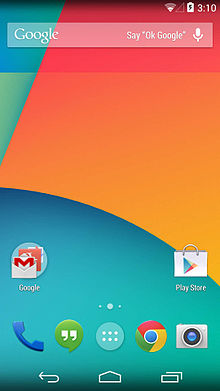
\includegraphics[width=4.95cm]{Bilder/Android4.jpg}
\caption{Android 4.4 Startbildschirm des Nexus 5 in Originalgr\"o\ss{}e \cite{WikiAndroid}}
\label{Der MongoDB-Chooser-Dialog}
\vspace{-20pt}
\end{wrapfigure}
Nach der Ver\"offentlichung des Android \ac{SDK} wurde 2008 mit dem "`G1"' das erste Smartphone mit dem neuen Betriebssystem Android vorgestellt. Ein direkten Vergleich zwischen Android und den von Apple stammenden iOS ging, zu dieser Zeit, klar zu Gunsten der Apple-Produkte aus.
% 
% Dem zu der Zeit noch Marktbeherschenden iOS und den iPhones, konnte 
 
Durch eine schnelle und konsequente Entwicklung konnten, der Firma Apple mit ihrem iOS, immer mehr Marktanteile abgenommen werden. Zum heutgen Zeitpunkt ist die Android-Plattform mit fast 85 Prozent Marktanteil im Bereich der Smartphonebetriebssysteme f\"uhrend. \cite{GolemMobileBetriebssystem}

Hardwarehersteller d\"urfen seit einiger Zeit nicht nur die Oberfl\"ache, sondern auch das Betriebssystem an sich auf ihre ganz speziellen Anforderungen anpassen, was zu einer gro\ss{}en Vielfalt der Plattform f\"uhrte. Ein pures unbearbeitetes Android ist zur Zeit nur auf Ger\"aten der "`Nexus-Reihe"' zu finden, welche zwar von verschiedenen Herstellern gebaut aber von Google vermarktet werden. Dies hat zur Folge das Systemupdates, auf Nexus-Ger\"aten, schneller und regelm\"a\ss{}iger zur Verf\"ugung stehen, da keine Anpassungen an den Updates, durch die Hardwarehersteller, vorgenommen werden m\"ussen.

Android ist momentan in der Version 4.4.4 alias "`Kit Kat"' auf dem Markt. Die Versionsnamen von Android sind immer nach einer S\"u\ss{}speise benannt und kommen in alphabetischer Reihenfolge auf den Markt. So folgte auf "`Jelly Bean"' die aktuelle Version Kit Kat. Eine nun schon in der Entwicklervorschau erschienene Version wird also mit "`L"' beginnen, weshalb diese Version momentan auch "`Android L"' genannt wird. Gut zu sehen ist, dass auf den Buchstaben J ein K folgte, welcher wiederum vom L abgel\"ost wird. \cite{WikiAndroid} \cite{Jung13}

Zus\"atzlich wurde dem Trend der "`Smartwatches"' folgend, im M\"arz 2014, ein speziell f\"ur Smartwatches angepasstes Android-System ver\"offentlicht, welches "`Android Wear"' hei\ss{}t. In dieser Arbeit wird jedoch nicht weiter auf Android Wear eingegangen, da dieses System nur im Zusammenspiel mit einem Smartphone in der Lage ist SMS zu empfangen. \cite{NextAndroidWear}

\subsection{Die Entwicklungsumgenung f\"ur Android}
Das schon angesprochene \ac{SDK} beinhaltet die folgenden Bestandteile:
\begin{itemize}
 \item Die eigentliche Entwicklungsumgenung mit Plugins
 \item Biblioteken und APIs
 \item Das Android Virtual Device
 \item Den USB-Treiber 
 \item Den SDK-Manager
 \item Das Programm dx
 
\end{itemize}

Nach dem downloaden und installieren der Android \ac{SDK} sind die eben genannten Bestandteile auf dem Rechner vorhanden und im Installationsverzeichnis zu finden. Die meisten Entwickler verwenden die \ac{IDE} Eclipse, f\"ur die eigentliche Programmierarbeit. Die im \ac{SDK} vorhandene Version von Eclipse enth\"alt das Plugin \ac{ADT}, welches viele Werkzeuge f\"ur die Android-Entwicklung mitbringt und welche sp\"ater genauer erl\"autert werden.

Eine andere Version des Android \ac{SDK} das sogenannte "`Android Studio"' bassiert auf der \ac{IDE} "`IntelliJ"'. Android Studio besitzt einige zus\"atzliche Features, wie die erweiterte "`Android Code-Completion"' oder die "`Multiple-APK generation"', welche es erlaubt eine Applikation gleichzeitig f\"ur Android und Android Wear zu erzeugen. Trotz der Vorteile, befindet sich das Android Studio noch in einer Beta-Phase und wird daher f\"ur die Entwicklung der App nicht verwendet. \cite{DevAndroidStudio}

Au\ss{}er der \ac{IDE} beinhaltet das Android \ac{SDK} die aktuellen Bibliotheken und APIs, welche f\"ur die Erstellung einer Applikation ben\"otigt werden. Dies beinhaltet auch Klassen, mit dessen Hilfe die zus\"atzliche Hardware in Android-Ger\"aten, wie das Notification-Light, angesprochen werden kann. Des weiteren ist auch eine lauff\"ahige Version des Androidbetriebssystems, welches f\"ur das Virtual Device ben\"otigt wird, vorhanden.

Das Virtual Device simuliert ein Smartphone am Rechner, auf dem die erstelle Applikation ausgef\"uhrt und getestet werden kann. Hierbei werden vom Virtual Device Debug-Information zur \ac{IDE} \"ubertragen, welche von dort aus angeschaut und ausgewertet werden k\"onnen.

Um eine geschriebene Applikation letztendlich nicht nur auf virtuellen Ger\"aten zu testen wird, unter Windows, ein USB-Treiber ben\"otigt. Dieser Treiber erm\"oglicht es, die Applikation auf ein reales Android-Ger\"at zu \"ubertragen und von dort aus zu Debuggen.
Um dies mit realer Hardware zu Testen, muss im entsprechenden Smartphone die "`Entwickler-Option"' aktiviert werden. Wie dies gemacht wird, wird im Kapitel ????? genauer beschrieben.

Der SDK-Manager ist ein Tool, mit dem die einzelnen Android-Version, Bibliotheken, APIs und Eclipse-Plugin-Versionen verwaltet und aktualisiert werden k\"onnen. Dies ist zum Beispiel hilfreich, wenn man eine Applikation unter verschiedenen Android-Version testen oder lauff\"ahig halten will.

Mit dem Namen dx wird ein Compiler bezeichnet, welcher Javaklassen unter Android lauff\"ahig macht. Mehr hierzu ist im folgenden Abschitt zu finden

\subsection{Dalvik anstelle der Java Virtual Machine}
Da eine Applikation f\"ur Android in Java geschrieben wird, liegt es nahe das auch hier eine virtuelle Maschine genutzt wird, welche ein Programm aus f\"uhrt. Im Android-System ist dies die \ac{DVM}, welche die Applikationen ausf\"uhrt.\cite{Android44}

\"Ahnlich wie die \emph{Java Virtual Machine} arbeitet auch Dalvik. Jedoch mit dem gro\ss{}en Unterschied, das Dalvik vom Google-Entwickler Dan Bornstein erdacht wurde um speziell auf leistungsschwachen mobilen Endger\"aten zu funktionieren.

Dalvik ist speziell daf\"ur entwickelt auf Prozessoren mit ARM-Architektur zu arbeiten, wobei die virtuelle Dalvik Maschine hier, im Gegensatz zur Java VM, in der Lage ist Hardwareregister direkt anzusprechen und zu nutzen. Durch die direkte Kommunikation mit der Hardware ergibt sich eine schnellere Verarbeitung des Codes als unter der Java VM direkt.

In der Theorie ist somit jede Javaklasse die unter Dalvik l\"auft auch unter der Java VM lauff\"ahig. Jedoch ergeben sich, in der Praxis, hier meist Schwierigkeiten durch Ein- und Ausgaben, da sich diese beim PC und Touchscreen grundlegend unterscheiden.

\subsubsection{Das Sandbox Prinzip}
Um Sicherheitsaspekten zu gen\"ugen besitzt Dalvik eine sogenannte Sandbox-Funktion, welche es erm\"oglicht Programme getrennt voneinander ausf\"uhren zu k\"onnen. F\"ur jedes auszuf\"uhrende Programm wird, unter Dalvik, eine neue Runtime-Umgegung erstellt, in der das Programm isoliert von anderen arbeitet. 
Dieses Prinzip wird Sandbox genannt, ja jedes Programm nur in seinem eigenen Sandkasten (Sandbox) "`spielen"' kann.

Dieses Vorgehen bringt sowohl Vorteile als auch Nachteile mit sich. Vorteilhaft ist, dass ein Programm nicht auf ein anderes zugreifen kann und dieses ungewollt ve\"andert, oder Daten aus einer anderen Programmausf\"uhrung abgreift. Gleichzeitig ist dieser Vorteil aber auch ein gro\ss{}er Nachteil, da ein gew\"unschter Austausch von Daten ebenfalls unterbunden wird.
Wie eine Daten\"ubertragen dennoch m\"oglich ist, wird im Kapitel ????? genauer behandelt.

\subsubsection{Von *.java zu *.dex}
Nachdem eine Javaklasse geschrieben wurde muss diese \"uber den Javacompiler (javac) in einen *.class-File umgewandelt werden. Dieser Class-File ist in der Theorie von jeder Java VM ausf\"uhrbar. Da die Klasse jedoch unter Dalvik optimiert laufen soll, muss sie ein weiteres mal Kompiliert werden. Diese zweite Kopilierungsstufe wird von dem schon erw\"ahnten Tool dx \"ubernommen. 
Der Dalvik-Compiler dx wandelt einen Class-File in einen von der \ac{DVM} ausf\"uhrbaren .dex-File um.

Dieser Zusammenhang ist in der Abbildung \ref{JavaZuDex} \"uber der Linie noch einmal zu sehen, da der beschriebene Zusammenhang auf dem Entwicklungsrecher passiert.

\begin{figure}[!ht]
\centering
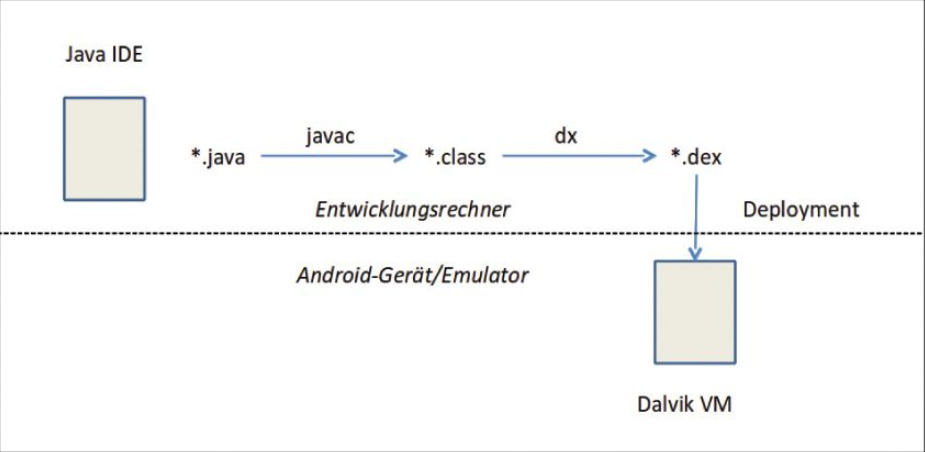
\includegraphics[width=12cm]{Bilder/JavaZuDex}
\caption{Von *.java zu *.dex \cite{Android44}}
\label{JavaZuDex}
\centering
\end{figure}
\newpage
\section{Bevor es losgehen kann - PC und Smartphone einrichten}
Bevor es mit der eigentlichen Programmierarbeit losgehen kann, muss zuerst das schon erw\"ahnte Android \ac{SDK}, von der Google-Developer-Seite\footnote{\url{http://developer.android.com/sdk/index.html}} heruntergeladen und installiert werden. Ist dies erledigt, kann es eigentlich schon fast losgehen.

\subsection{Der Android SDK Manager} \label{Der Android SDK Manager}
Bevor die Programmierarbeit losgehen kann muss nach der installation zuerst der "`Android SDK Manager"' gestartet werden. Dies ist zum einen wichtig, um die neusten Updates zu laden, aber auch um die passenden APIs zu laden.

Wie schon erw�hnt, ist der Manager zum einen die Update-Plattform des \ac{SDK}-Packets und zum anderen auch der Installer f�r neue Packete.

Beim starten des \ac{SDK} Managers werden Updates f�r schon installierte Packete angeboten. Damit der Download und die Installation startet, muss der Nutzer diesen Vorgang best�tigen. Sind alle Updates geladen und werden keine neuen Packete ben�tigt kann der Manager wieder geschlossen werden.

Beim ersten Starten des Managers muss aber noch ausgew�hlt werden auf welchem API-Level (welcher Android-Version) programmiert werden soll. Da Android relativ weit abw�rtskompatibel ist, empfiehlt es sich bei einem neuen Projekt immer die neuste API zu installieren. 

Durch die Verwendung der neusten API ist zum einen garantiert, dass das Projekt auf der neusten Android-Version l\"auft, zum anderen ist sichergestellt, dass das Projekt relativ lange ohne \"Anderungen mit zuk\"unftigen Versionen lauff\"ahig bleibt.
\newpage
\section{Der grundlegende Aufbau einer Android App}
Im nun folgenden Kapitel wird der grundlegende Aufbau einer Android App genauer beschrieben, wobei auf wichtige Bestandteile im Projekt eingegangen wird.
Zum einen soll hier der zugrundeliegende Dateiaufbau aber auch die Bestandteile einer App und deren Funktion genauer erl\"autert dargestellt werden. \cite{Android44}

\subsection{Componenten einer Applikation aus Sicht des Nutzers}
Eine App unter Android bestizt aus der sicht des Nutzers vier Hauptbestandteile:
\begin{itemize}
 \item Activity
 \item Broadcast Receiver
 \item Service
 \item ContentProvider
\end{itemize}

\subsubsection{Die Activity} \label{Die Activity aus Nutzersicht}
Eine Activity, unter Android, ist eine Benutzeroberfl\"ache in der App, wobei ein Projekt beliebig viele Activitys haben kann. Somit sind Activitys im eigentlichen Sinn Fenster, die in der Regel den gesamten Bildschirm f\"ullen und eine gewisse Aufgabe erf\"ullen. \cite{Kuehn12}

Der Aufruf verschiedener Activitys kann entweder vom Programmablauf vorgegeben sein oder durch Nutzeraktionen variieren. So kann zum Beispiel jenachdem welchen Button der Nutzer bet\"atigt eine andere Activity aufgerufen werden. \cite{Android44}

Eine Activity hat einen bestimmten Lebenszyklus den sie im Verlauf der Anwendung durchl\"auft. Beim erstellen einer Activity wird als erstes die Methode \texttt{onCreate} aufgerufen. Jenachdem welche Folgeaktion der Nutzer als n\"achstes ausf\"uhrt wird eine der Anderen Methoden wie im Bild \ref{ActivityLebenszyklus} aufgerufen. Wird die Activity wieder beendet, so wird die Methode \texttt{onDestroy} aufgerufen. 

Inaktiv ist eine Activity zum Beispiel dann, wenn die von einer anderen komplett oder Teilweise \"uberdeckt wird. Sollte eine neue Activity \"uber der alten ge\"offnet werden, wird diese nicht sofort zerst\"ort, sondern auf einer Art Stack gehalten von woaus sie wieder aufgerufen werden kann. Dies w\"are der Fall, wenn der Nutzer die Zur\"ucktaste bet\"atigt.

Activitys die sich im Stack befinden, werden erst gel\"oscht, wenn die zugeh\"orige App geschlossen oder Arbeitsspeicher freigegeben werden muss. 

Alle im Bild \ref{ActivityLebenszyklus} zu sehenden Methoden sind in der Tabelle \ref{Lebenszyklus-Methode einer Activity} im Kapitel \ref{Die Activity aus Programmierersicht} noch einmal genauer beschrieben.

\begin{figure}[!ht]
\centering
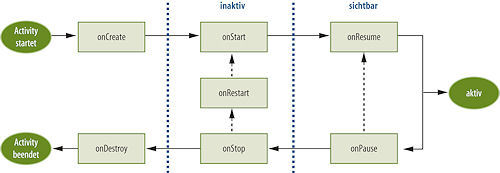
\includegraphics[width=12cm]{Bilder/ActivityLifecycle}
\caption{Der Lebenszyklus einer Activity \cite{ActivityLifecycle}}
\label{ActivityLebenszyklus}
\centering
\end{figure}
\FloatBarrier

% In der folgenden Tabelle sind alle m\"oglichen Methoden beschrieben, welche im Lebenszyklus einer Activity vom Betriebssystem aufgerufen werden k\"onnen.

\subsubsection{Broadcast Receiver} \label{Broadcast Receiver aus Nutzersicht}
Ein Broadcast Receiver unter Android ist ein Empf\"anger f\"ur verschiedene Benachrichtigungen die vom Betriebssystem abgesetzt werden. Benachrichtigungen unter Android sind vielf\"altig und k\"onnen zum Beispiel bei erhalt einer SMS oder E-Mail gesendet werden. Alle im System registrieten Receiver werden bei ihrem zugeh\"origen Event aktiv und bleiben dies auch nur f\"ur die Zeit, welche es ben\"otigt die Methode \texttt{onReceive} auszuf\"uhren.

Android unterscheidet grunds\"atzlich zwei verschiedene Arten von Broadcast Receivern und zwar Dynamische und Statische Broadcast Receiver. Dynamische Broadcast Receiver sind nicht im System registriert und k\"onnen nur zur Laufzeit der Komponente (Activity oder Service) auf Ereignisse reagieren. Statische Broadcast Receiver hingegen m\"ussen im Betriebssystem registriert werden. Hierf\"ur m\"ussen sie in der Manifest-Datei deklariert sein, wie eine Manifest-Datei aufgebaut ist, ist im Kapitel \ref{Die Manifest-Datei} genauer beschrieben. Durch die Regisitrierung im System muss die zugeh\"orige App nicht laufen um einen Broadcast zu empfangen und zu verarbeiten.

\subsubsection{Services} \label{Services aus Nutzersicht}
Services in Android sind gedacht f\"ur Programmbestandteile, welche keine Benutzeroberfl\"ache ben\"otigen. Hintergrundprozesse, wie zum Beispiel das abspielen von Musik oder das herunterladen von Daten sind typische Anwendungsf\"alle f\"ur Services. 

Wie schon bei den Broadcast Receivern gibt es im Androidsystem zwei Arten von Services, zum einen den Loacl Service welcher an eine bestimmte Komponente gebunden ist und zum anderen Remote Services, welche in einem eigenen Prozess laufen auch nachem die App beendet wurde.

\subsubsection{ContentProvider} \label{ContentProvider aus Nutzersicht}
ContentProvider sind Schnittstellen f\"ur die \"Ubergabe von Daten oder Datenbankeintr\"agen an andere App.
Greift eine App zum Beispiel auf das Telefonbuch des Smartphones zu, geschieht dies \"uber einen ContentProvider. Daten werden durch die ContentProvider anderen Apps zur verf\"ugung gestellt werden, wobei immer nur der Dateninhalt und nicht die Datei selbst \"ubergeben wird. \cite{Kuehn12}

ContentProvider sind wie eben schon einmal erw\"ahnt gewisse Daten aus der applikationseigenen Datenbank durch eine Art Schaufenster darzustellen und sie bei bedarf zu \"ubergeben.

\subsection{Componenten einer Applikation aus Sicht des Programmierers}
Eine App besteht f\"ur den Programmierer nat\"urlich aus sehr viel mehr als nur die vier f\"ur den Nutzer sichtbaren Teile. Welche das sind und welche Aufgaben sie haben ist im folgenden genauer beschrieben. \cite{GolemHBAppAusEntwicklerSicht}

\subsubsection{Der Projektbaum}
\cite{GolemHBRessourcen}

\subsubsection{Die Manifest-Datei} \label{Die Manifest-Datei}
Das Android Manifest ist die Schaltzentrale einer App, in der alle Bestandteile einer Applikation aufgef\"uhrt sind. Das Manifestunter Android ist also XML-Datei im Wurzelverzeichnis abgelegt. 

Im Manifest sind als erstes Informationen zum Package-Name zu sehen (1) welche direkt vor der Versionsnummer und dem Versionsnamen zufinden sind (2). Unter \texttt{uses-sdk} ist zum einen die Angabe zur minimalen Android-Version angegeben und zum anderen mit welcher Version Kompiliert wurde (3). \texttt{uses-permission} gibt an, welche Berechtigungen die App in anspruch nimmt (4). Zum Schluss m\"ussen nat\"urlich auch noch alle Activitys und Services angegeben werden (5).
\cite{Android44}

Im Listing ist eine Manifest-Datei beispielhaft zu sehen.

\lstinputlisting{Code/ManifestExample.xml}

\subsubsection{Das Rechtekonzept in Android}

\subsubsection{Intents} \label{Intents}
Wie im Verlauf dieses Kapitels schon gezeigt wurde sind App's unter Android komponentenorientiert aufgebaut, was bedeutet das die einzelnen Komponenten wie Activitys, Services, BroadcastReceiver und ContentProvider untereinander kommunizieren m\"ussen. Hier kommen die Intents ins Spiel, welche die Aufgabe haben Nachrichten und Daten unter den Komponenten einer App aber auch systemweit zu \"ubermitteln und im gleichen Zug eine andere Activity zu starten.

Android unterscheidet zwei verschiedene Arten von Intents, zum einen den "`Expliziten Intent"' und zum anderen den "`Impliziten Intent"'. Explizite Intents sind f\"ur die Kommunikation innerhalb einer App relevant, da hier explitit eine andere Komponente aufgerufen wird. 

Im Listig wird ein neuer Intent gebaut, welcher zum einen den Context, also die aufrufende Komponente und zum anderen eine zweite Activity (\texttt{SecondActivity}) aufruft. Mittels der Methode \texttt{startActivity} wird der Intentent, also die andere Activity gestartet.

\lstinputlisting{Code/ExpliziterIntentExample.java}

Implizite Intents sind f\"ur die App\"ubergreifende Kommunikation gedacht, wobei hier ein Intent erstellt wird in der Hoffnung, dass eine App diese Inhalte \"offnen kann.
Im Listig wird beispielhaft ein Intent erstellt, welcher dem Nutzer Daten anzeigen soll. Dies geschieht mit \texttt{Intent.ACTION\_VIEW}, wobei als Uri ein String mit Koordinaten f\"ur eine Karte mit \"ubertragen wird.

\lstinputlisting{Code/ImpliziterIntentExample.java}

Das Betriebssystem schaut nun welche installierten App's diesen Kontent verarbeiten k\"onnen und gibt bei mehreren M\"oglichkeiten dem Nutzer eine Wahlm\"oglichkeit um selbst zu bestimmen mit welcher App der Kontent dargestellt werden soll.

Damit das Betriebssystem jedoch weis, welche Impliziten Intents von einer App verarbeiten werden k\"onnen m\"ussen sogenannten "`Intent Filter"' im Manifest angegeben werden.
Im Manifest m\"ussen alle Komponenten registriert werden, so auch die Activitys einer App. In der Angabe zur Activity kann zus\"atzlich ein Intent Filter hinzugef\"ugt werden, welcher angibt, das diese spezielle Activity in der Lage ist Intents zu verarbeiten.

Im Listing wird nur der Manifest-Ausschnitt mit der betreffenden Activity gezeigt (1), wobei diese einen Intent Filter besitzt der einen View \"offnet (2). Zus\"atzlich zur Aktion wurde noch eine entsprechende Kategorie angef\"ugt, welcher den Intent weiter eingrenzt (3). \cite{VogellaIntent}

\lstinputlisting{Code/ImpliziterIntentManifestExample.xml}

\subsubsection{Die Activity} \label{Die Activity aus Programmierersicht}
Activitys sind wie im Kapitel \ref{Die Activity aus Nutzersicht} schon dargestellt die Benutzeroberfl\"ache, welche der Nutzer sieht, und mit der er Interagieren kann.

Eine Activity-Klasse erbt von der Android-API-Klasse \texttt{ActionBarActivity} und hat die in der Tabelle \ref{Lebenszyklus-Methode einer Activity} aufgef\"uhrten wichtigen Methoden, welche sie von der Oberklasse erbt.

% \FloatBarrier
\begin{table}[!ht]
\begin{tabular}{|p{3cm}|p{12cm}|}
 \hline Methode & Beschreibung \\
 \hline onCreate & Diese Methode wird beim erzeugen der Activity aufgerufen und kann wie ein Konstruktor verwendet werden. Es werden alle Felder, Formulare, Men\"us und Layouts hier initialisiert.\\&\\
 onStart & Wird ausgef\"uhrt, wenn die Activity neu erzeugt wird oder sie aus dem Hintergrund wieder hervortritt, wie es zum Beispiel beim dr\"ucken der Zur\"ucktaste der Fall ist.\\&\\
 onResume & Wenn eine teilweise verdeckte Activity wieder in den Focus r\"uckt wird diese Methode Aufgerufen.\\&\\
 onPause & Diese Methode wird Ausgef\"uhrt, wenn die Activity teilweise verdeckt wird und somit inaktiv wird.\\&\\
 onStop & Wird ausgef\"uhrt, wenn die Activity in den Hintergrund tritt und auf den Stack abgelegt wird.\\&\\
 onRestart & Die Activity r\"uckt vom Stack wieder in den Vordergrund weil diese wieder ben\"otigt wird.\\&\\
 onDestroy & Diese Methode wird ausgef\"uhrt, wenn die Activity beendet wird. In ihr sollten alle belegten Ressourcen wieder freigegeben werden.\\
 \hline
\end{tabular}
\caption{Lebenszyklus-Methode einer Activity \cite{Android44}}
\label{Lebenszyklus-Methode einer Activity}
\end{table}
\FloatBarrier

\subsubsection{Broadcast Receiver} \label{Broadcast Receiver aus Programmierersicht}
Eine Broadcast-Receiver-Klasse erbt von der Android-API-Klasse \texttt{BroadcastReceiver}. Ein Broadcast Receiver erbt nur die Methode \texttt{onReceive} welche Ausgef\"uhrt wird, wenn ein Broadcast empfangen wird. Hieraus wird auch ersichtlich, das ein Broadcast Receiver nur zur Zeit der Ausf\"uhrung existiert.

Um einen Statischen Receiver im Manifest einzutragen wird ein Eintrag in der Manifest-Datei ben\"otigt, wie im Listing unten beispielhaft f\"ur einen Receiver der auf das Event \texttt{BOOT\_COMPLETED} reagiert dargestellt ist. Dieser Receiver wird ausgef\"uhrt, wenn das System fertig gebootet hat. Zum einen wird der Name der Receiver-Klasse eingetragen (BootReceiver), zum anderen auf welchen Intent er reagieren soll (im Beispiel \texttt{BOOT\_COMPLETED}).

\lstinputlisting{Code/BroadcastReceiverManifest.xml}

Ein Dynamischer Broadcast Receiver wird einfach innerhalb einer Javaklasse zum Beispiel einer Activity aufgerufen und ist dann f\"ur die Lebensdauer der Komponente aktiv. Wird die Komponente geschlossen kann der Receiver folglich nicht mehr reagieren.

\subsubsection{Services} \label{Services}
Wie schon im Kapitel \ref{Services aus Nutzersicht} vorgestellt, gibt es unter Android die Local Services und die Remote Services. Beide Arten m\"ussen in der Manifest-Datei aufgef\"uhrt werden, wobei ein Local Servie nur mit dem Klassenname angegeben werden muss, wie das Listing zeigt. Der Klassenname des Service ist im Beispiel "`DatabaseService"', der Punkt sagt aus, dass sich die Klasse im selben Verzeichnis wie das Manifest befindet.

\lstinputlisting{Code/LocalServiceManifest.xml}

Ein Remote Service ben\"otigt zus\"atzlich zum Klassennamen noch einen Prozessnamen, da der Service ja in einem eigenen Prozess starten soll. Das Listig vom Local Service muss also im den Prozessnamen erweitert werden.

Der Doppelpunkt vor dem Namen (im Listing "`MyDatabaseService"') sagt aus, dass der Service in einem eigenen Prozess starten soll.

Sollte der Servicename mit einem Gro\ss{}buchstaben beginnen, so l\"auft er unter dem selben User wie die App selbst und kann somit nur von der App angesprochen werden, da wie im Kapitel \ref{Das Sandbox Prinzip} beschrieben jede App unter einem anderen User l\"auft. Beginnt der Servicename jedoch mit einem Kleinbuchstaben so l\"auft er global und kann von jeder App angesprochen werden.

\lstinputlisting{Code/RemoteServiceManifest.xml}

Ein Local Service wird mit der Methode \texttt{startService} gestartet und besitzt die folgenden Lebenszyklus-Methoden wie sie in der Tabelle \ref{Lebenszyklus-Methode eines Local Service} aufgef\"uhrt sind.

% \FloatBarrier
\begin{table}[!ht]
\begin{tabular}{|p{3cm}|p{12cm}|}
 \hline Methode & Beschreibung \\
 \hline onCreate & Diese Methode wird beim erzeugen des Service  und kann wie ein Konstruktor verwendet werden. Sie sollte f\"ur Initialisierungen genutzt werden.\\&\\
 onStartCommand & Wird aufgerufen, wenn die Methode \"uber \texttt{Context.startService} gestartet wird und ist neu seit Android 2.0.\\&\\
 onDestroy & Diese Methode wird aufgerufen, wenn der Service beendet wird, wobei ein Service sich auch \"uber die Methode \texttt{stopSelf} selbstst\"andig beenden kann.\\
 \hline
\end{tabular}
\caption{Lebenszyklus-Methode eines Local Service \cite{Android44}}
\label{Lebenszyklus-Methode eines Local Service}
\end{table}
\FloatBarrier

Ein Remote Service wird an eine Activity gebunden und wird \"uber die Methode \texttt{bindService} gestartet. In der Tabelle \ref{Lebenszyklus-Methode eines Remote Service} sind die Lebenszyklus-Methoden eines Remote Services.

\FloatBarrier
\begin{table}[!ht]
\begin{tabular}{|p{3cm}|p{12cm}|}
 \hline Methode & Beschreibung \\
 \hline onCreate & Wie in Tabelle \ref{Lebenszyklus-Methode eines Local Service}.\\&\\
 onBinde & Wird aufgerufen, sobald sich eine Komponente mit dem Service Verbindet und gibt eine Instanz vom Typ \texttt{IBinder} zur\"uck.\\&\\
 onUnbinde & Wird aufgerufen, wenn die Komponente die Verbindung zum Service beendet.\\&\\
 onDestroy & Wie in Tabelle \ref{Lebenszyklus-Methode eines Local Service}.\\
 \hline
\end{tabular}
\caption{Lebenszyklus-Methode eines Remote Service \cite{Android44}}
\label{Lebenszyklus-Methode eines Remote Service}
\end{table}
\FloatBarrier

\subsubsection{ContentProvider}
ContentProvider sind wie im Kapitel \ref{ContentProvider aus Nutzersicht} schon erw\"ahnt in der Lage, Dateiinhalte \"uber Applikationsgrenzen hinweg zu durchzureichen.

Ein ContentProvider erbt von der abstrackte Klasse \texttt{ContentProvider} aus der Android-API und muss mindestens die vier Methoden \texttt{query}, \texttt{insert}, \texttt{update} und \texttt{delete}. \"Uber diese Methoden ist es m\"oglich Daten zu bekommen und gegebenen falls zu manipulieren. Nat\"urlich m\"ussen die Daten \"uberhaupt erst mal gefunden werden, bevor sie gelesen oder ge\"andert werden k\"onnen, dies geschieht \"uber die Methode \texttt{getContentResolver}. \cite{Kuehn12}

Der Lebenszyklus eines ContentProvider ist \"ahnlich dem eines Broadcast Receivers, da er nur erstellt wenn er wirklich ben\"otigt wird. Sollte auf einen Provider zugegriffen werden, dessen App nicht l\"auft, wird dieser vor dem Aufruf vom Betriebssystem erstellt.

Da das Thema der ContentProvider jedoch sehr gr\"o\ss{} ist, kann es hier nicht in allen Einzelheiten erl\"autert werden. 

\subsection{Google-APIs} \label{Google-APIs}
\cite{GolemHBGoogleServices}


\end{spacing}




\newpage
\section{Abk�rzungsverzeichnis}
\begin{acronym}
  \acro{SDK}{\emph{Software Development Kits}}
  \acro{OHA}{\emph{Open Handset Alliance}}
  \acro{IDE}{\emph{Integrierte Entwicklungsumgebung}}
  \acro{ADT}{\emph{Android Development Tools}}
  \acro{DVM}{\emph{Dalvik Virtual Machine}}
  \acro{FME}{\emph{Funkmeldeempf\"anger}}
  \acro{JIT}{\emph{Just in Time}}
  \acro{ART}{\emph{Android Runtime}}
  \acro{AOT}{\emph{Ahead-of-Time-Decodierung}}
  \acro{API}{\emph{Application Programming Interface}}
  \acro{}{\emph{}}
%  \acro{KIT}{\emph{Karlsruher Instituts f�r Technologie}}
%  \acro{GDS}{\emph{Generic Data Services}}
% %  \acro{LSDF}{\emph{Large Scale Data Facility}}
%  \acro{OPM}{\emph{Objektorientierten Programmiermodell}}
%  \acro{SMD}{\emph{Strukturelle Metadaten}}
%  \acro{JSON}{\emph{JavaScript Object Notation}}
% %  \acro{HALO}{\emph{High Altitude and Long Range Research Aircraft}}
%  \acro{IAI}{\emph{Institut f�r Angewandte Informatik}}
%  \acro{JAXB}{\emph{Java Architecture for XML Binding}}
%  \acro{UDDE}{\emph{User Data Description Editor}}
%  \acro{AMD}{\emph{Anwendermetadaten}}
%  \acro{CG}{\emph{Class Generator}}
%  \acro{IG}{\emph{Interface Generator}}
\end{acronym}
\newpage
\listoffigures
% Abk�rzungsverzeichnis
\newpage
\bibliographystyle{alpha}
% verzeichnis im DIN format
\bibliography{Quellen}
\end{document}
